\documentclass{thesisclass}
% Based on thesisclass.cls of Timo Rohrberg, 2009
% ----------------------------------------------------------------
% Thesis - Main document
% ----------------------------------------------------------------
% No empty in-between chapters, remove this line if desired for double-page printing
%\let\cleardoublepage\clearpage


\newcommand{\til}{{\raise.17ex\hbox{$\scriptstyle\mathtt{\sim}$}}}

\usepackage{mathtools}
\usepackage{pdfcomment}
\usetikzlibrary{decorations.pathreplacing,angles, quotes, calligraphy, fit, shadings}
\usepackage{tikzpagenodes}

\newcommand{\bigO}{\mathcal{O}}

\usepackage{lineno}
\makeatletter
\def\makeLineNumberLeft{%
  \linenumberfont\llap{\hb@xt@\linenumberwidth{\LineNumber\hss}\hskip\linenumbersep}% left line number
  \hskip\columnwidth% skip over column of text
  \rlap{\hskip\linenumbersep\hb@xt@\linenumberwidth{\hss\LineNumber}}\hss}% right line number
\leftlinenumbers% Re-issue [left] option
\makeatother

\linenumbers

\usepackage{xargs}                      % Use more than one optional parameter in a new commands
%\usepackage[pdftex,dvipsnames]{xcolor}  % Coloured text etc.

\usepackage[colorinlistoftodos,prependcaption,textsize=tiny]{todonotes}
\newcommandx{\unsure}[2][1=]{\todo[linecolor=red,backgroundcolor=red!25,bordercolor=red,#1]{#2}}
\newcommandx{\change}[2][1=]{\todo[linecolor=blue,backgroundcolor=blue!25,bordercolor=blue,#1]{#2}}
\newcommandx{\info}[2][1=]{\todo[linecolor=OliveGreen,backgroundcolor=OliveGreen!25,bordercolor=OliveGreen,#1]{#2}}
\newcommandx{\improvement}[2][1=]{\todo[linecolor=Plum,backgroundcolor=Plum!25,bordercolor=Plum,#1]{#2}}
\newcommandx{\thiswillnotshow}[2][1=]{\todo[disable,#1]{#2}}

\setlength{\marginparwidth}{20mm}

\usepackage{booktabs}
\newcommand{\ra}[1]{\renewcommand{\arraystretch}{#1}}


\usepackage{subcaption}
\usetikzlibrary[spy,calc]

\usepackage{pgf}
\usepackage{acronym}

\usepackage{footnote}
\usepackage{svg}

\makesavenoteenv{tabular*}
\DeclareMathOperator*{\argmax}{arg\,max}
\DeclareMathOperator*{\argmin}{arg\,min}

\DeclarePairedDelimiter\abs{\lvert}{\rvert}%
\DeclarePairedDelimiter\norm{\lVert}{\rVert}%

\usepackage{calc}

\usepackage[export]{adjustbox}

\usepackage{algorithm}
\usepackage[noend]{algpseudocode}

\makeatletter
\def\BState{\State\hskip-\ALG@thistlm}
\makeatother

\pdfinclusioncopyfonts=1
\usepackage[activate={true,nocompatibility}]{microtype}

\newcommand{\dif}{\mathop{}\!\mathrm{d}}

\usepackage{amssymb}
\usepackage{placeins}


%% -------------------------------
%% |  Information for PDF file   |
%% -------------------------------
\hypersetup{
 pdfauthor={Andreas Mikolajewski},
 pdftitle={Efficient datastructures and sampling of many light sources for Next Event Estimation},
 pdfsubject={Photon-based Next Event Estimation},
 pdfkeywords={Computer graphics, photorealism, path tracer, Next Event Estimation, importance sampling}
}


%% ---------------------------------
%% | Information about the thesis  |
%% ---------------------------------

\newcommand{\myname}{Andreas Mikolajewski}
\newcommand{\mytitle}{Efficient datastructures and sampling of many light sources for \\Next Event Estimation}
\newcommand{\myinstitute}{KIT Computer Graphics}

\newcommand{\reviewerone}{?}
\newcommand{\reviewertwo}{?}
\newcommand{\advisor}{?}
\newcommand{\advisortwo}{?}

\newcommand{\timestart}{XX. Monat 20XX}
\newcommand{\timeend}{XX. Monat 20XX}
\newcommand{\submissiontime}{DD. MM. 20XX}

%% --------------------------------
%% | Settings for word separation |
%% --------------------------------
% Help for separation:
% In german package the following hints are additionally available:
% "- = Additional separation
% "| = Suppress ligation and possible separation (e.g. Schaf"|fell)
% "~ = Hyphenation without separation (e.g. bergauf und "~ab)
% "= = Hyphenation with separation before and after
% "" = Separation without a hyphenation (e.g. und/""oder)

% Describe separation hints here:
\hyphenation{
% Pro-to-koll-in-stan-zen
% Ma-na-ge-ment  Netz-werk-ele-men-ten
% Netz-werk Netz-werk-re-ser-vie-rung
% Netz-werk-adap-ter Fein-ju-stier-ung
% Da-ten-strom-spe-zi-fi-ka-tion Pa-ket-rumpf
% Kon-troll-in-stanz
}


%% ------------------------
%% |    Including files   |
%% ------------------------
% Only files listed here will be included!
% Useful command for partially translating the document (for bug-fixing e.g.)
\includeonly{
titlepage,
content,
chapters/abstract,
chapters/introduction,
chapters/fundamentals,
chapters/previouswork,
chapters/PNEE,
chapters/implementation,
chapters/evaluation,
chapters/prospect,
chapters/appendix,
acronym
}

\makeatletter

\newrobustcmd*{\parentexttrack}[1]{%
  \begingroup
  \blx@blxinit
  \blx@setsfcodes
  \blx@bibopenparen#1\blx@bibcloseparen
  \endgroup}

\AtEveryCite{%
  \let\parentext=\parentexttrack%
  \let\bibopenparen=\bibopenbracket%
  \let\bibcloseparen=\bibclosebracket}

\makeatother

\addbibresource{thesis.bib}

%%%%%%%%%%%%%%%%%%%%%%%%%%%%%%%%%
%% Here, main documents begins %%
%%%%%%%%%%%%%%%%%%%%%%%%%%%%%%%%%
\begin{document}

\frontmatter
\pagenumbering{roman}
\include{titlepage}
\blankpage

\chapter*{Abstract}

Modern photorealistic media production faces an increasing number of light sources to produce natural-looking images. A very significant percentage of processing time goes towards casting shadow rays to calculate the direct lighting term with Next Event Estimation. Naively sampling many light sources in a path tracer quickly becomes impractical, as our evaluation shows. We present a novel technique to importance sample many light sources called Photon-based Next Event Estimation (PNEE). In a preprocess,  similar to photon mapping, photons are scattered from all light sources into the scene. These photons are used to build cumulative distribution functions (CDF) that reflect the importance of the light sources to reduce the variance of Monte Carlo Integration. We evaluate several storage options and data structures for efficient lookups within the integrator. We introduce and utilize two novel data structures to store CDFs: sparse CDFs and interpolated CDFs. To mitigate variance edges and artifacts, we present several interpolation and approximation techniques. We evaluate several variants of PNEE against naive NEE as well as PBRTs recent implementation, and demonstrate that even for moderately complex scenes a 50-100x speedup can be achieved.
%% -------------------
%% |   Directories   |
%% -------------------
\listoftodos[Notes]
\tableofcontents
\blankpage


%% -----------------
%% |   Main part   |
%% -----------------
\mainmatter
\pagenumbering{arabic}
%% ==============================
\chapter{Introduction}
\label{ch:Introduction}
%% ==============================

There are generally two utilized families of algorithms to render a picture from a scene description: rasterization and ray tracing. With rasterization, you start with the objects and splat them onto the view frustum. This performs very well and with various extending techniques creates very good looking, but not necessarily physically correct, results.  Rasterization is very common for real-time applications and graphics card pipelines are highly optimized for it. On the other hand ray tracing is usually considered slow and runs on the CPU\footnote{Exceptions and new advancements exist, see for example NVIDIA RTX.}, so use cases are more limited, but actually tracing light paths from light sources to the lens is a necessity to allow for physically correct and unbiased estimation of a scenes light transport.

Because of the quite intricate nature of light itself (e.g. wave-particle dualism) it is not really possible to solve the light transport equation with a basically infinite number of dimensions. The solution is to explore as many, hopefully important, light paths as possible with each decision for the path construction done probabilistically. For each event that gets chosen by a random variable, the result is later divided by the probability of its occurrence. More specifically the continuous integrals are estimated with the Monte Carlo integration, allowing the estimation of a continuous function with only a limited number of samples. We describe these concepts in more detail in chapter~\ref{ch:Fundamentals}.

When constructing the paths there are many choices and considerations one can take. Should you start at the eye or the light source, or both and later connect the path segments? How to compute the reflection on a surface? How does the medium affect the current path and refraction? Can you adjust the probabilities based on a preprocess or guide paths based on preceding path calculations?
These questions spark a variety of techniques and sub-techniques, our Photon-based Next Event Estimation (PNEE) is one of them. Acknowledging the existence and possible suitability of techniques like Bidirectional Path-tracing (BDPT), Metropolis light transport and others, throughout this work we focus our discussion only on path tracing without loss of applicability to the aforementioned.

With path tracing each path is started at the eye and only one refraction is considered at each intersection. The depth of the path is commonly limited by Russian Roulette (RR). For each pixel, a multitude of paths are started from random positions within the pixel (providing free Anti-aliasing). Aside from the single main path which covers indirect lighting, it is very effective to use Next Event Estimation (NEE) at every intersection point. NEE does estimate the direct lighting by deterministically connecting each intersection point to a light source. The rendering equation can be split up into a direct and indirect lighting part to enable this without introducing bias (see section~\ref{sec:NEE}).

With an ever-expanding complexity of modeled scenes, the presence of many light sources greatly contributes to a natural and appealing image. Choosing the most contributing light sources for NEE thus gets more and more important, with modern path tracers taking up to 50\% of today's rendering time for direct lighting calculations, mainly because evaluating the visibility term is costly. Many lights usually lead to many occluded respectively localized light influences. As the incident light integral is estimated with finitely many samples with Monte Carlo Integration the variance of this estimation is greatly dependant on how well the sampling probabilities fit the estimated function. For this reason, estimating good probability density functions (PDF) over the importance of light sources is a promising topic for research.

In this work, we present a novel technique, Photon-based Next Event Estimation (PNEE). The idea is to scatter out photons from the light sources and use them to build up a data structure which later can be used to build a PDF within the integrator. There are several design decisions that can be made through the phases of PNEE.

\begin{itemize}
    \item how to shoot photons
    \item what to store
    \item which acceleration data structure to use
    \item how to interpolate the result
\end{itemize}

For each of this phases, we explore several sub-techniques, combine them and evaluate them against each other as well as other established techniques for NEE. We achieved speedups between 50-100x in balanced test scenes, with the efficiency further scaling up as the lighting complexity of the scene increases. Nonetheless, all techniques have their own special kinds of artifacts that may not show up in the MSE but can be very irritating for a human observer. We mitigate these problems effectively and present strong results within three different test scenes that cover a high range of lighting situations.

\unsure{The source code is probably nice. Should I exclude the masterthesis repo though? It is the latex code of the document.}
\blfootnote{
All sources, test scenes, test results and images can be found at:

\begin{itemize}
    \item \url{https://github.com/AndiMiko/pbrt-v3}
    \item \url{https://github.com/AndiMiko/pbrt-scenes}
    \item \url{https://github.com/AndiMiko/PNEE-data}
    \item \url{https://github.com/AndiMiko/masterthesis} 
\end{itemize}
}
%% ==============
\chapter{Fundamentals}
\label{ch:Fundamentals}
%% ==============

\section{Raytracer}


%% ==============
\section{Rendering equation}

\subsection{Light Path Expressions}
\subsection{Measurement Contribution Function}


%% ==============
\section{Sampling}

\subsection{Probablity Density Function}

\subsection{Cumulative Distribution Function}

\subsection{Inverse Transform Sampling}

\subsection{Monte-Carlo Integration}

\subsection{Importance Sampling}

\subsection{Multiple Importance Sampling}

%% ==============
\section{Bidirectional scattering distribution function}
% mainly only for introduction of specular vs diffuse reflections


%% ==============
\section{Light sources}


%% ==============
\section{Path Tracing}
\subsection{Next Event Estimation}



%% ==============
\section{Photon Mapping}

\subsection{Progressive Photon Mapping}

\subsection{Stochastic Progressive Photon Mapping}



%% ==============
\section{Instant Radiosity}

%% ==============
\section{Datastructures}

% Teapot in a stadium ...

\subsection{Bounding Volume Hierarchy}
\subsection{Grid}
\subsection{Octree}
\subsection{k-d Tree}
\subsection{Surface Area Heuristic}


%% ==============
\chapter{Related Work}
\label{ch:Prev}
%% ==============

We introduced academic fundamentals that we base our work on in the previous section. In this chapter, we further evaluate both past and recent work that focuses specifically on handling many light sources. Some work of late explicitly targets Next Event Estimation, while similar problems can also be found in work about Instant Radiosity \parencite{keller1997instant, Walter2005LightcutsAS, dachsbacher2014scalable}. Due to the large number of virtual point lights, several techniques had been developed to scale sublinearly. We have to be cautious when taking these techniques into account, as one of our main goals is to remain unbiased; most work on Instant Radiosity is dependent on biased approximations.

\paragraph{Early work}

Early work on this topic from \textcite{ward1994adaptive} sorts light sources by power and tests them sequentially up until a cutoff.  \textcite{Shirley:1996:MCT:226150.226151} later improve this by introducing the construction of probability distribution functions (PDF) for simple area light shapes. Sampling within an area light is a problem on its own but is well understood for basic shapes. They then describes how those PDFs can be combined to inherit multiple light sources. \citeauthor{Shirley:1996:MCT:226150.226151} also discuss weighting the sampling probability of the light sources uniformly and based on energy, which produce reasonable results in simple scenes but quickly breaks down with many light sources and occlusion. This is, in essence, the technique we later refer to as \textit{power} in chapter~\ref{ch:Evaluation} discussions. They then further propose a technique to spatially divide the scene with an octree to account for more localized influences. Still, these calculations remain based on light power, angle, and spatial distance and fail to attribute for any kind of occlusion.

\textcite{DBLP:conf/vmv/KellerW00} extend photon mapping to utilize its already existing photon map for importance sampling. The proposed algorithm only roughly classifies light sources into two importance groups and then importance samples accordingly. For the generation single photons are used; we later show in chapter~\ref{ch:Evaluation} that this is not feasible, despite introducing several improvements in chapter~\ref{ch:PNEE}. \textcite{DBLP:conf/rt/WaldBS03} propose an approach for interactive applications. A crude path tracer preprocessing step is utilized. With a downsized resolution light, importance PDFs are precached in screen space. 

\paragraph{Lightcuts}

\textcite{DBLP:journals/cgf/PaquettePD98} are one of the first to introduce a light hierarchy (tree) which can be used to move down in detail until approximated criteria are met. This concept is extended upon and adapted to Instant Radiosity by \textcite{Walter2005LightcutsAS} in their landmark paper introducing Lightcuts. A Lighttree hierarchically combines the light sources of a scene. The leaves are light sources which get pooled into clusters by position and orientation. A Lightcut, in turn, is a set of nodes such that a path from any leaf to the root will contain exactly one node from the cut. We discuss how Lightcuts might be applied to PNEE in section~\ref{sec:lightcutd}.

More recent work from \textcite{Estevez} is inspired by Lightcuts and ports some ideas to unbiased Next Event Estimation for many lights. Just like in Lightcuts, a Lighttree is constructed. Later, to choose a light source, a cut is calculated by moving down the clusters as long criteria for position and normal cone orientation are met. All lights found below the cut are then sampled uniformly or based on energy.

\paragraph{Grid caching}

\textcite{Vevoda} propose a technique which also utilizes a Lighttree and Lightcuts but combines it with a world space cache. The scene is subdivided into a regular grid where each cell holds a cut of the Lighttree. Similar to \citeauthor{Estevez}, this cut can be used to importance sample given light sources. Noteworthy is that a cut is lazily calculated only when a shading point within an empty cell is rendered, but can later be reused for all shading points within the same grid cell.

By coincidence, PBRT \parencite{pbrt}, the renderer we use throughout this work, recently committed a similar (yet undocumented) technique to its Github repository. It is not mentioned in edition three of the book but likely will appear in its next edition. Comments indicate that such a technique was crucial to be able to render scenes with many lights like Zero-Day, which we also use for comparison in chapter~\ref{ch:Evaluation}. \citeauthor{pbrt} do not use Lightcuts. Instead, usual PDFs are constructed, but the algorithm for lazy world space caching in a grid is very similar to \citeauthor{Vevoda}'s technique.

To elaborate, whenever a shading point is rendered within a grid cell that is not yet cached, 128 random points within the cell are sampled and deterministically connected to all light sources (a random point for area lights). Based on the position, distance, and orientation of the light, an average importance weight for any light source is calculated and a PDF is constructed. In its current state, occlusion is wholly ignored. However, a comment in the code indicates, that there is or was an attempt to include occlusion; we discuss this further in section~\ref{sec:pbrtoccl}. We continue to refer to the technique as it is internally referred to: \textit{Spatial}.

\paragraph{Reinforcement learning}

\parencite{DBLP:journals/corr/DahmK17} utilize machine learning in their recent work which details how light transport paths are more generally learned by a $\mathcal{Q}$-function with reinforcement learning. The $\mathcal{Q}$-functions are distributed in screen space and form a Voronoi diagram which guides sampling.

\paragraph{Outlook}

Just recently before the publication of this work \textcite{Vevoda:2018:BOR} present an extension of their previous work. A Bayesian online learning algorithm is utilized to gradually learn occlusion into the initially naively constructed Lightcut cache. We continue our discussion on this work in section~\ref{sec:pbrtoccl}.

%% ==============
\chapter{Photon-based Next Event Estimation}
\label{ch:PNEE}
%% ==============

We propose a novel approach to find estimators for importance sampling (especially) for scenes with many localized light sources. Our key goal is to efficiently reduce the variance $\sigma$ (section~\ref{sec:IS}) \unsure{ref to sections?} of the direct lighting term of our Monte Carlo integrator (section~\ref{sec:MC}) by estimating the strength of the light contribution from every light source. Typically ruling out light sources that contribute nothing (zero contribution paths) due to shadowing has a significant impact.

In a preprocess all light sources scatter out photons into the scene, similar to photon mapping \cite{jensen2001realistic}, but no bounces are considered, as we only need direct light paths for our Next Event Estimation estimator. Further, we only consider LD paths, all LS*D paths are disregarded. Those paths are disregarded by the first condition anyway, but we want to emphasize that refractions of any kind make a photon obsolete for our usecase. After the photons are scattered out into the scene we are looking for efficient ways to approximate or store those photons. Contrary to techniques like proposed by \cite{Estevez} where we build up our datastructures around the light sources themselves, with PNEE we build the datastructures around the light-receiving parts of our scene. This generally will scale up the data that needs to be processed but at the same time bear opportunity to refine our estimators. Then, the last step happens from within our pathtracer, we produce an estimator for our Next Event Estimation at every intersection by accessing and processing surrounding photons or CDFs.

Note that when the photon count goes towards infinity and the intersection search radius goes towards zero the estimator becomes the direct lighting term we are trying to find, making the Monte Carlo integration obsolete. As we are bound by time and memory, the key challenge is to find a good approximation thereof in minimal time. We found that shooting, processing and storing photons in the preprocess is not as tightly bound, but the lookup thereof in the integrator is very timecritical as it runs once for each intersection in the pathtracer. In the following sections we discuss various datastructures and storing methods we explored throughout this work.



\section{Mix and match}

Throughout this work we explored several techniques that trade off time, memory and image quality (visible artifacts)\footnote{As all our techniques are unbiased, images always converge against the same result. In practice those artifacts converge almost never, thus we list artifacts, even though they just can be seen as huge time tradeoff.}. From a meta-perspective we can divide our technique into several subprocesses:

\begin{itemize}
    \item shoot photons (section~\ref{ch:shootph})
    \item store those photons in some form (section~\ref{ch:formofstorage})
    \item add this information into a fitting acceleration datastructure (section~\ref{ch:AccelDat})
    \item and finally, from within the path tracer, retrieve this information and potentially interpolate it to construct meaningful estimators (section \ref{ch:interpolation})
\end{itemize}

For each subprocess we present several ideas, where mostly any permutation of those ideas could be utilized. Unsurprisingly, there are several natural fits, which we describe in more detail, have implemented and evaluate against each other and known techniques in section~\ref{ch:Evaluation}. We refer to the implemented techniques as \textit{cdfgrid}, \textit{photontree} and \textit{cdftree}. All of which have specific peculiarities and parameters which are introduced during the course of this work. Table \ref{tb:techniques} gives an overview of subtechniques and colors indicate which of those are implemented with the respective technique. We advise the reader to refer back to this overview, to put newly introduced techniques into perspective.
\unsure{good table and styling?}

\begin{center}


\newcommand{\tdot}[1]{ \tikz\draw[#1,fill=#1] (0,0) circle (.5ex); }
\ra{1.3}
\begin{tabular}{@{}llll@{}}\toprule
shooting photons & form of storage & acceleration datastructure & interpolation \\ \midrule

uniform \tdot{yellow}\tdot{blue}\tdot{green}        & photons \tdot{blue}               & hashed grid \tdot{yellow}                 & none \tdot{yellow}\tdot{blue}\tdot{green}\\
powerbased \tdot{yellow}\tdot{blue}\tdot{green}     & lightcuts                         & k-d tree \tdot{blue}\tdot{green}          & trilinear \tdot{yellow} \\
other strategies                                    & CDFs \tdot{yellow}\tdot{green}    &                                           & shepard \tdot{blue}\tdot{green}\\
\bottomrule
\multicolumn{4}{c}{cdfgrid \tdot{yellow} \qquad photontree \tdot{blue} \qquad cdftree \tdot{green}} 
\end{tabular}
%\captionof{table}{Various subtechniques introduced throughout this work. Colors indicate which subtechnique was implemented with the respective technique. }
\label{tb:techniques}
\end{center}




\section{Shooting photons}
\label{ch:shootph}
The first step in the preprocess is to scatter out photons. We rely on the same theoretical basis as photon mapping (section \ref{sec:PM}) but without producing any kind of bias as long as our CDFs always inherit every light source. We generate photons at the scenes light sources and intersect them with our scene geometry. We sample the light source $x$ and a point s and direction $\omega$ on that light source with respect to a probability distribution. This bears opportunity to guide the generation of photons to maximize the photon density in the important parts of the scene. Let $L(s,\omega)$ be the radiance \unsure{radiance?} at point s in direction $\omega$, $p(x)$ the probability to sample light source $x$ and $p(\text{s}, \omega)$ the probability to sample the ray, the energy $\beta$ of this photon is calculated as follows.

\begin{equation}\label{eq:beta}
\beta = \frac{|\cos{\omega}|L(\text{s}, \omega)}{p(x)p(\text{s}, \omega)}
\end{equation}

The basic approach is to use uniform CDFs to sample both $p(x)$ and $p(\text{s}, \omega)$. We found that results can be greatly enhanced for typical (but not all) scenes by sampling $x$ based on the light power. We elaborate differences in section \ref{ch:}\todo{input section}. In the future it might be of value to migrate sampling strategies presented for photon mapping to PNEE, see \cite{DBLP:conf/rt/SuykensW00}\todo{add more}. After we found the first intersection of the photon we check the surface BSDF, if it is fully specular, the photon can be discarded, if it has a diffuse part we store the photon, or at least its origin and $\beta$ in a data structure which we discuss in the next sections.

\section{Form of storage}
\label{ch:formofstorage}

\subsection{Photons}

Storing every photon with its weight and potentially additional data like the direction it came from is the most precise form to later compute our estimator, as the number of datapoints corresponds to our photon count. For every intersection point we evaluate the surrounding photons and compute an individual cumulative distribution function. As the photon count is quite high, typically several million unevenly distributed datapoints, the lookup is a bottleneck in this case, even with acceleration structures like a k-d tree that we discuss in section~\ref{sec:pneekdtree}. Nonetheless, the approach is worthwhile due to the potential quality of the estimator.

If we want to lessen the strain on the integrator, we might reduce the number of datapoints within the preprocess and store an approximation instead of every individual photon. We accumulate the $\beta$ per light sample $x$ within a defined area. Then this map of weights is transformed into a lightcut or CDF.

\subsection{Lightcut}

Recent work from Estevez and Kulla \cite{Estevez} and Vévoda and Křivánek \cite{Vevoda} rely on lightcuts. A lightcut is a horizontal cut through a lighttree (essentially a binary tree with light sources as leafs) and has the advantage of being very compact when many adjacent leafs of the subtree have the same sampling probability. This is quite typical, as most of the times only a small portion of lights contribute to a given point, while all other lights are shadowed. Let $n$ be the number of lights and $c$ the size of the cut. $c$ can be anything between one, cutting once at the root node, and $n$, cutting each leaf. Lightcuts thus adapt to the complexity of the given datapoint and often can be stored quite compact. Sampling from such a cut runs in $\bigO(\log{n})$ but on avarage in $\bigO(\log{c})$, size of the lighttree is $\bigO(n\log{n})$. The advantages of lightcuts break down when there are none or few adjacent samples that share the same probability. Proposed algorithms by Estevez \cite{Estevez} and others to find such a cut, in our view, have similarities to unsupervised machine learning algorithms, where the lighttree is a dendrogram of a cluster (typically produced by agglomerative hierarchical clustering) and the algorithm tries to assign a label (the probability) to the lights based on their cluster affinity. 

\subsection{CDF}

Another possibility is to directly store cumulative distribution functions during the preprocess. A CDF is usually stored as an sorted array of float values that grow from 0 to 1, the size is fixed at $n$, and sampling is done in $\bigO(\log{n})$. With our technique we found lightcuts not well fitting, as rather than making broad approximate statements about clusters of lights, we dominantly have individually distinct contributions accumulated through photons. Let $k$ be the number of contributing light sources to a particular CDF, which equals to all light sources with a sampling probability unequal to zero. This would degenerate a lightcut into a CDF where $c \approx k$. Especially when creating CDFs within the integrator a linear space and timecomplexity is generally unacceptable. We observe that most of the time $k$ is significantly smaller than $n$ due to localized light influences. To address this issue we present Sparse CDFs in section~\ref{sec:sparse} where space- and time complexity for construction is $\bigO(k)$ and sampling is $\bigO(\log{k})$. Furthermore, in section \ref{sec:intcdf} we introduce the possibility to sublinearly interpolate between any kind of CDFs in $\bigO(d)$ space and time for construction and $\bigO(d + \log{n})$ sampling, where $d$ is the number of interpolated CDFs.
%TODO: Wie tief soll ich hier gehen wieso das so ist?

\subsubsection{Sparse CDF}
\label{sec:sparse}
\begin{figure}[htb] 
	\centering
    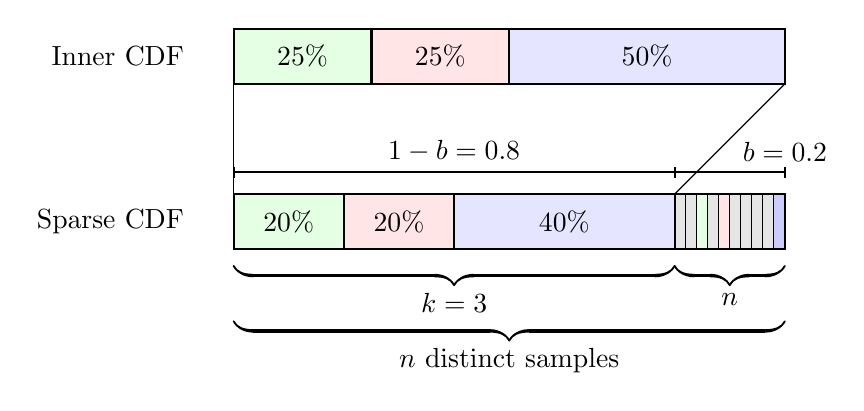
\begin{tikzpicture}[scale=7, cdf/.style ={thick}]

    
    %zoom lines
    \draw (0,0) -- (0,-0.2);
    \draw (1,0) -- (0.8,-0.2);
    

    %cdfs, lines and filling
    \draw[thick, fill=green!10] (0,0) rectangle (0.25, 0.1) node[pos=.5] {25\%};
    \draw[thick, fill=red!10] (0.25, 0) rectangle (0.5, 0.1) node[pos=.5] {25\%};
    \draw[thick, fill=blue!10] (0.5, 0) rectangle (1, 0.1) node[pos=.5] {50\%};
    
    \draw[thick, fill=green!10] (0, -0.3) rectangle (0.2, -0.2) node[pos=.5] {20\%};
    \draw[thick, fill=red!10] (0.2, -0.3) rectangle (0.4, -0.2) node[pos=.5] {20\%};
    \draw[thick, fill=blue!10] (0.4, -0.3) rectangle (0.8, -0.2) node[pos=.5] {40\%};
    
    \draw[thick, fill=black!10] (0.8, -0.3) rectangle (1, -0.2);
    
    \fill[fill=green!10] (0.84, -0.3) rectangle (0.86, -0.2);
    \fill[fill=red!10] (0.88, -0.3) rectangle (0.9, -0.2);
    \fill[fill=blue!20] (0.98, -0.3) rectangle (1, -0.2);
    
    \foreach\x in {0.82,0.84,...,0.98}
        \draw (\x,-0.2) -- (\x,-0.3);
        
    \draw[cdf] (0,0) rectangle node[left=4cm] {Inner CDF} (1,0.1);
    \draw[cdf] (0,-0.3) rectangle node[left=4cm] {Sparse CDF} (1,-0.2);
    
    % b range indicators
    \draw[thick] (0, -0.16) -- node[above] {$1-b = 0.8$} (0.8, -0.16) ;
    \draw[thick] (0, -0.17) -- (0, -0.15);
    
    \draw[thick] (0.8, -0.16) -- (1, -0.16) node[above] {$b = 0.2$} ;
    \draw[thick] (0.8, -0.17) -- (0.8, -0.15);
    \draw[thick] (1, -0.17) -- (1, -0.15);
    
    % braces
    \draw[line width=1.25pt, decoration={calligraphic brace,amplitude=7pt,mirror,raise=6pt},decorate]
                    (0,-0.3) -- node[below=12pt] {$k = 3$} (0.8,-0.3);
    \draw[line width=1.25pt, decoration={calligraphic brace,amplitude=7pt,mirror,raise=6pt},decorate]
                    (0.8,-0.3) -- node[below=12pt] {$n$} (1,-0.3);
    \draw[line width=1.25pt, decoration={calligraphic brace,amplitude=7pt,mirror,raise=26pt},decorate]
                    (0,-0.3) -- node[below=32pt] {$n$ distinct samples} (1,-0.3);

\end{tikzpicture}
    \caption{A sparse CDF either samples from the uniform part with probability $b$ or from the inner CDF with probability $1-b$. $k$ are the number of samples that have a non-zero probability in the non-uniform part. All $k$ samples are repeated within the uniform part to facilitate calculations of $p_{\text{sparse}}$ (equation \ref{eq:psparse}). The samples in sparse CDF are not in the correct order, as a result two additional hashmaps are needed.} 
    \label{fig:sparseCDF}
\end{figure}

We need \unsure{we need?} a CDF where only particular values from $0$ to $n$ may be sampled. We achieve this by using a classic CDF (inner CDF) with length $k$ and a hashmap which maps values $[1,k]\to [1,n]$\footnote{As the pre-image in $[1,k]\to [1,n]$ is a sequence this could also be a simple array instead of a hashmap. Before constructing the sparse CDF the photons are collected by some algorithm without knowing $k$ beforehand. As photons can originate from all $n$ light sources a hashmap is needed anyway. We continue with this hashmap to spare the conversion.}. After we sampled a number the map will map the sampled number to the original sample number. Further we also need a backmap which is the reverse of the former map. The backmap is used when you want to know the probability of a given original sample number $x$. The original sample number is mapped to the sample number that it corresponds to in the inner CDF, so the inner CDF can be queried for the corresponding probability. We additionally want to provide a base floor probability $b$, which is split equally by all $n$ light sources. Let $N$ be the set of all $n$ sample numbers and $K$ be the set of non-zero probability samples. The probability that a given sample $x$ is sampled by the sparse CDF is given as follows.
\begin{equation}\label{eq:psparse}
 p_{\text{sparse}}(x) = 
\begin{dcases}
    p_{\text{inner}}(\text{backmap}(x))(1 - b) + \frac{b}{n},& \text{if } x \in K\\
    \frac{b}{n}, & \text{otherwise}
\end{dcases}
\end{equation}
Even though we seemingly introduce unnecessary variance with this uniform base, it is absolutely crucial as we otherwise would introduce bias whenever our estimator would "forget" a light source, which is not uncommon for e.g. very distant or highly occluded light sources. Apart from that fact, it generally helps in areas where our estimator is bad for any reason, therefore the choice of $b$ should not be minimal, but rather roughly proportional to the expected quality of the estimator.

Construction is done in $\bigO(k)$ space and time, sampling in $\bigO(\log{k})$. Comparing to lightcuts we have a simpler datastructure in hand, that rules out non contributing light samples effectively. If we assume that equal non-zero probabilities are rare, which should be the case with many photon contributions, we generally should outperform lightcuts, especially because sampling the dominant case $x \notin K$ runs in $\bigO(1)$. 

\subsubsection{Interpolated CDF}
\label{sec:intcdf}
\begin{figure}[htb] 
	\centering
    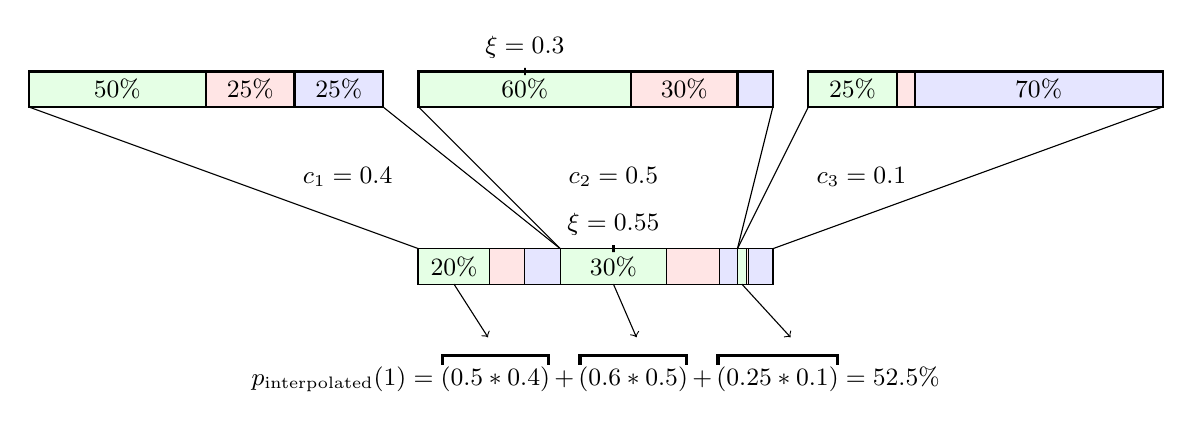
\begin{tikzpicture}[scale=4.5, cdf/.style ={thick}]
    \small
    %zoom lines
    \draw (-1.1,0) -- (0,-0.4);
    \draw (-0.1,0) -- (0.4,-0.4);
    \draw (0,0) -- (0.4,-0.4);
    \draw (1,0) -- (0.9,-0.4);
    \draw (1.1,0) -- (0.9,-0.4);
    \draw (2.1,0) -- (1,-0.4);
    
    \draw[cdf] (-1.1,0) rectangle (-0.1,0.1);
    \draw[cdf] (0,0) rectangle (1,0.1);
    \draw[cdf] (1.1,0) rectangle (2.1,0.1);
    \draw[cdf] (0,-0.5) rectangle (0.4,-0.4);
    \draw[cdf] (0.4,-0.5) rectangle (0.9,-0.4);
    \draw[cdf] (0.9,-0.5) rectangle (1,-0.4);
    
    %cdfs, lines and filling
    \draw[thick, fill=green!10] (-1.1,0) rectangle (-0.6, 0.1) node[pos=.5] {50\%};
    \draw[thick, fill=red!10] (-0.6, 0) rectangle (-0.35, 0.1) node[pos=.5] {25\%};
    \draw[thick, fill=blue!10] (-0.35, 0) rectangle (-0.1, 0.1) node[pos=.5] {25\%};
    
    \draw[thick, fill=green!10] (0,0) rectangle (0.6, 0.1) node[pos=.5] {60\%};
    \draw[thick, fill=red!10] (0.6, 0) rectangle (0.9, 0.1) node[pos=.5] {30\%};
    \draw[thick, fill=blue!10] (0.9, 0) rectangle (1, 0.1);
    
    \draw[thick, fill=green!10] (1.1,0) rectangle (1.35, 0.1) node[pos=.5] {25\%};
    \draw[thick, fill=red!10] (1.35, 0) rectangle (1.4, 0.1);
    \draw[thick, fill=blue!10] (1.4, 0) rectangle (2.1, 0.1) node[pos=.5] {70\%};
    
    \draw[fill=green!10] (0,-0.5) rectangle (0.2,-0.4) node[pos=.5] {20\%};
    \draw[fill=red!10] (0.2,-0.5) rectangle (0.3,-0.4);
    \draw[fill=blue!10] (0.3,-0.5) rectangle (0.4,-0.4);

    \draw[fill=green!10] (0.4,-0.5) rectangle (0.7,-0.4) node[pos=.5] {30\%};
    \draw[fill=red!10] (0.7,-0.5) rectangle (0.85,-0.4);
    \draw[fill=blue!10] (0.85,-0.5) rectangle (0.9,-0.4);
    
    \draw[fill=green!10] (0.9,-0.5) rectangle (0.925,-0.4);
    \draw[fill=red!10] (0.925,-0.5) rectangle (0.93,-0.4);
    \draw[fill=blue!10] (0.93,-0.5) rectangle (1,-0.4);
    
    \draw[thick] (0.55,-0.39) node[above] {$\xi = 0.55$} rectangle (0.55,-0.41);
    
    \draw[thick] (0.3, 0.11) node[above] {$\xi = 0.3$} rectangle (0.3,0.09);
    
    \node at (0.5, -0.75) {$p_{\text{interpolated}}(1) = \overbracket{(0.5 * 0.4)} + \overbracket{(0.6 * 0.5)} + \overbracket{(0.25 * 0.1)} = 52.5\%$};
    
    \draw[->] (0.1,-0.5) -- (0.196,-0.65);
    \draw[->] (0.55,-0.5) -- (0.615,-0.65);
    \draw[->] (0.9125,-0.5) -- (1.05,-0.65);
    
    % pi range indicators
    \path (-0.2, -0.25) node[above] {$c_1 = 0.4$};
    \path (0.55, -0.25) node[above] {$c_2 = 0.5$};
    \path (1.25, -0.25) node[above] {$c_3 = 0.1$};
    
\end{tikzpicture}
    \caption{Three CDFs should be interpolated with corresponding weights $c_i$. Randomnumber $\xi$ is $0.55$. The second CDF is chosen, $\xi$ is cut and normalized to $0.3$. Sample 1 (green) is chosen. $p_{\text{interpolated}}$ is calculated according to equation \ref{eq:pinter}.} 
    \label{fig:interpolatedCDF}
\end{figure}

Suppose we want to sample a number from an interpolation between $d$ CDFs. A naive approach to achieve this is to loop through every CDF and for every sample add up the weights, normalize them in the end and store this as the new interpolated CDF. Construction would then run in $\bigO(d * n)$ and $\bigO(n)$ space, sampling in $\bigO(\log{n})$. As we will need the construction to run for every intersection in our scene it is unsustainable to have it run linearly in $n$. We propose a CDF interpolation scheme that constructs in $\bigO(d)$ time and space, with only minimal drawback when sampling with $\bigO(d + \log{n})$.

We receive a list of CDFs to interpolate and corresponding weights. We loop through the weights and normalize them, thus constructing an usual CDF that will sample $i \in [1,d]$. We keep an array of references to the base CDFs. Now, for the lookup we sample $i$ in $\bigO(\log{d})$ and then choose the $i'th$ CDF and sample within the CDF in $\bigO(\log{n})$. We now have the sample $x$ and also have to calculate the probability that $x$ was sampled. Let $c_i$ be the probability to sample the $i'th$ CDF and $p_i(x)$ the probability of sampling $x$ within the $i'th$ CDF, we calculate the probability as follows.

\begin{equation}\label{eq:pinter}
    p_{\text{interpolated}}(x) = \sum_{i=1}^{d}p_{i}(x) \cdot c_i
\end{equation}

The time complexity for this calculation is $\bigO(d)$, resulting in overall complexity $\bigO(\log{d} + \log{n} + d) = \bigO(d + \log{n})$. The whole process is illustrated in figure \ref{fig:interpolatedCDF}. Note that with our construction all base CDFs are required to have the same number of samples $n$ in the exact same order. This restriction might be lifted with additional maps, similar to sparse CDFs, but we have no need for it, as all our used CDFs have the same $n$ lights, thus we spare the overhead.

\section{Acceleration datastructure}
\label{ch:AccelDat}

After choosing what we store we are choosing how we store and access it from within our integrator. A critical part of finding our estimator is to access the data we previously stored. It is important to keep the probable distribution of photons in mind. Usually large parts of the scene won't have any photons and then there will be photon clusters, typically distributed on 3D-planes. Further, a typical problemcase for the choice of acceleration datastructures is called "teapot in a stadium" \todo{illustration?}. It describes the potentially vastly varying level of detail in a scene. The "teapot" is a small, highly detailed object in the "stadium" which is big, simple and mostly empty. This bears a typical trade off between adaptive datastructures like octrees or k-d trees, which handle varying LOD quite well, but generally have slower access times and static datastructures like a hashed grid, which has fast constant access times, but can't adapt to LOD at all. For our renderer often times not even the big $\bigO$ runtime is critical, but the constant overhead can be problematic, too. The best choice is often scene dependent, nonetheless, we are trying to find a good middleground that solves typical problem cases in photorealistic scenes. The form of storage does also impact the effectiveness of the acceleration datastructure, we present natural fits in the following chapters.

\subsection{Hashed grid}
\label{ch:pnee:hashedgrid}
Storing photons directly into a hashed grid is quite dangerous, almost any scene will have clusters of photons, sometimes consisting of a large portion of the total photon count. When doing a nearest neighbour lookup of our intersection point this can degenerate to linear run time complexity, not even in the light source count $n$, but in the total photon count. It is apparent that this is unacceptable, as even a small detail in the scene could blow up rendering times.

The idea here is to store exactly one CDF in the middle of each grid cell and using the clamped position as the key. Doing so, we utilize the constant access times of the hashed grid without the threat of photon clusters. At the same time we are giving up precision, as we loose all positional data of the photons. We do not interpolate the photons by distance to the CDF, rather every photon contributes at the same rate to this homogeneous grid cell. As every intersection point will clearly choose one CDF, this leads to sometimes very apparent variance cliffs at the edges of the grid cells (see figure \ref{fig:varianceEdge}). PBRTs \cite{pbrt} and Vevodas \cite{Vevoda} \unsure{use cite here or ref to the section where I introduced the technique?} technique have the exact same problem, but their CDFs transition somewhat smoothly as only position and angles are used for CDF calculation. The problem is highly accelerated with our technique because we inherit occlusion in the CDF generation which can create sharp edges in certain situations. We tackle this problem in section \ref{ch:trilinear}.


\subsection{k-d tree}
\label{sec:pneekdtree}

A k-d tree does fit much better when it comes to storing photons in a scene with potentially high variance in LOD. Construction of the tree is well studied, we thus throughout this work relied on Nanoflann \cite{blanco2014nanoflann}\unsure{implementation detail ok here?}, a highly optimized C++ k-d tree framework. After the photons are stored in the tree, the time critical part happens from within the integrator. 

A k-d tree can be queried for it's nearest neighbours or a defined radius. We tried both techniques, which vary mostly on how we interpolate the photons to construct the CDF. A NN-lookup has the advantage that in sparsely populated areas enough photons are always count to construct a somewhat meaningful CDF. Imagine a very distant object where only a few photons land, a radius-lookup might produce sharp variance edges where no photons are found, compared to regions where one or a few photons are found. With the radius-lookup the radius instead of the photon count is fixed, this helps fine tuning the interpolation kernels and allows unlimited number of lights to influence a point. Imagine a point where several thousands lights influence it's shading, a NN-lookup would construct a CDF with at maximum the number of lights of nearest neighbours, not even accounting for photons from the same light source. Finding an arbitrary amount of photons within a radius might get a problem performance wise, too. In extreme cases we suffer from similar problems like a hashed grid with a fixed radius with worse lookup times. Either the choice of radius or nearest neighbours becomes a critical parameter for the described scenarios. As photon density also depends on total photon count, both parameters are also influenced by the total photon count, which further complicates the issue. Considering the fact, that it is rare that so many light sources influence a point and even if so, individual contributions are low and likely somewhat uniform\footnote{Strong light sources will also dominate in the photon count. So if photons are uniform the result will likely be uniform. But there may be exceptions to this with sharp angles or very spiky BSDFs.}, thus this drawback will rarely cause problems. Not knowing the radius can be handled by the interpolation scheme, where for example modified shepard (section \ref{sec:modshep}) adapts to the maximum radius to smoothly phase the furthest photon in and out. From a theoretical standpoint we expect NN-lookups to be the more stable technique, still both have their pitfalls. Further analysis on this behaviour is made in section \ref{ch:ev:photontree}.

No matter which lookup method we choose we have to collect the accumulated $\beta$ per light. If we want to avoid running linearly in the number of lights, we have to use a hashmap mapping from light number to its $\beta$ in combination with the sparse CDF (\ref{sec:sparse}). Let the number of collected photons be $u$. It quickly becomes apparent that this technique has a high precision, but suffers heavily from constant factors. Every intersection point collects $u$ photons, every photon is looked up in $\bigO(\log n)$\footnote{Much less in reality as the k-d tree backtracks and does not start from the root for every photon, but the constant factor $u$ is still a problem.}, then interpolated in constant time, hashed in constant time and several datastructeres have to be built for the sparse CDF, all of this may only be used exactly once for each intersection point. During our work, testing those constant factors, it became desirable to do more calculations and approximations during the preprocess that can be amortized throughout the rendering phase, but still preserve the capability to adapt to level of detail.

\subsubsection{Clustering}

To reduce the mostly constant factors of constructing CDFs just mentioned, we try to precompute and reuse those CDFs. In a sense this is comparable to the CDFs from section \ref{ch:pnee:hashedgrid}, but they can be placed at arbitrary locations and thus adapt to level of detail. This requires a completely different preprocess and interpolation methods due to the absence of a structured grid. To sharpen the difference of both techniques, in an ideal scenario where the clustering and interpolation does act as desired, we are essentially trading memory versus time complexity. If we want to increase the level of detail with a hashed grid, we have to increase the number of voxels into all three dimensions. Due to those three dimensions it does not scale well and becomes unfeasible at a certain point. Many CDFs are just empty somewhere in the air\footnote{Sparse CDFs help a lot with memory usage here. Even though big $\bigO$ memory complexity stays the same.}. With a k-d tree we can use the same amount of CDFs/memory where ever they are needed for LOD, but we are giving up the constant access times of a hashed grid. Nonetheless, a k-d tree does scale well with the number of CDFs in time and memory. As briefly mentioned, the difficult part is finding stable techniques for the preprocess and interpolation.

Our first intuition was to make a cluster analysis on the photons to find cluster centroids and cluster affinity for every photon. The centroids can then be used as CDFs where every photon from this cluster accumulate its $\beta$ into the CDF. We researched several machine learning techniques for clustering. Hierarchical clustering algorithms like AHC produce useful dendrogram which could be interesting to explore, but AHC, and many other clustering algorithms can quickly be ruled out due their time complexity of at least $\bigO(n^2)$. The only possibility is to do the analysis on a small subset of clusters, construct and store the CDFs into a k-d tree and then adding every other photon to it's closest CDF in $\bigO(\log k)$, where $k$ is the number of clusters. We found those approaches not stable enough, with a small subset scene details are quickly missed, with a bigger subset scaling becomes an issue. Also adding several million photons in $\bigO(\log k)$ is feasible but is still significant. Further, we have to produce spherical clusters, because photons will be reduced into their centroid, from where structural information is lost, only a spherical influence radius is retained from then on. See figure \ref{fig:clustering} for a comparison. Producing only hyper-sphere clusters is often considered a drawback of k-means clustering, but is exactly what we need in this case. Having to define the number of centroids beforehand is also not a problem for us.

We have done extensive tests with k-means clustering, but at first highly underestimated the amount of clusters we need to produce good results. K-means clustering with k-means++ seeding \cite{DBLP:conf/soda/ArthurV07} is considered one of the fastest clustering algorithms with a time complexity of $\bigO(nkdi)$ where $n$ is the number of $d$-dimensional data points, $k$ the number of clusters and $i$ the number of iterations needed to converge. This does work with several million photons and a few dozen clusters, but we found that a typical scene would at least need several thousand CDFs. With a high $n$ and high $k$ scaling quickly becomes a problem again. Quite recent work from \cite{DBLP:conf/kse/HieuM14}, \cite{DBLP:journals/tpds/XuQLMLL14} and \cite{DBLP:conf/www/Sculley10} introduced better scaling to k-means at the cost of slight approximations, which in fact shouldn't really bother us. We especially tried working with the mini-batch k-means algorithm, but once again, scaling was an issue. Our last attempt at a clustering algorithm was Birch \cite{DBLP:conf/sigmod/ZhangRL96} from the sci-kit learn machine learning library \cite{scikit-learn}. Coming closer to our needs, we still were bound by either time or memory, depending on the configuration, and couldn't manage to achieve desirable run times.

We don't bother very much for the exact cluster affinity of single photons, thus a good approximation of spatial subdivision should be enough. This is often not the case for machine learning purposes. Also the dimensionality is often higher. In fact, k-d trees offer exactly this spatial subdivision based on surface area heuristics in 3D but fail for higher dimensions. With a construction time of $\bigO(n \log n)$ they fit our scalability needs and we can configure how many photons our leafs should maximally have. There are still peculiarities like single photon leafs that we have to handle, we discuss this in section \ref{ch:ev:cdftree}. After the k-d tree is constructed we iterate each leaf, calculate the centroid of each leaf based on the contained photons and construct a CDF to place on that centroid. After all CDFs are constructed we construct a new k-d tree over all CDFs. This k-d tree is then later used for lookups from within the integrator in $\bigO(\log k)$.

Comparing to storing photons we reduced our lookup cost from $\bigO(\log n)$ to $\bigO(\log k)$ and the number of lookups can be significantly lower, as we only care about a smooth interpolation between the CDFs and don't have to worry about missing out on certain light sources. Additionally no hashes have to be computed, instead of a sparse CDF we are constructing an interpolated CDF, which has less overhead attached to it. Nonetheless, we are giving up precision and we are dependent on the quality of our preprocess and interpolation. We discuss interpolating unstructured data points in section \ref{ch:unstructured}.


\section{Interpolation}
\label{ch:interpolation}

In theory, a completely converged picture would always resemble the real light transport in the scene, one would not have to care about variance edges within the scene (as there is none). In practice, we are trying to find good estimators for our importance sampling to reduce processing time. This might work well for certain parts of the scene, but also has a chance to fail for other parts. If the estimator is bad, we sample the important part so rarely (see figure \ref{fig:importancesample}), that this parts might never, or at least extremely slowly, converge, thus sharp variance edges may occur. When the estimator is good for most parts and only bad a few times, this might not be captured by the mean squared error to the reference picture, but human perception is quite sensitive to this variance edges, see figure \ref{fig:varianceEdgeCdfgrid}. As Variance is the margin between estimator and estimated function, variance edges can occur for two reasons, either the estimator does change rapidly, or the scene does change rapidly. Changes of the estimator feel much more unnatural, as we see no apparent reason for those image artifacts, an actual change in the scene (like a hole you are looking through) might not be judged that harshly by a human observer, as the context does change - and with it, the variance\unsure{good?bad?}. With our techniques we always have some spatially precomputed data packets which constitute a discrete representation of our estimators. When estimators are chosen naively this discrete representation shows with unwanted variance edges. We need interpolation to turn this discrete data packets into a continuous and smooth function of estimators. We can't avoid variance in estimator quality, but we try to make it smooth and unnoticeable.

\begin{figure}[htb] 
	\centering
    %\captionsetup[subfigure]{labelformat=empty}

\begin{tikzpicture}[zoomboxarray, zoomboxarray columns=1, zoomboxarray rows=1]
    \node [image node] { \includegraphics[width=0.5\textwidth]{figures/test2_artifacts.png} };
    \zoombox[magnification=8,color code=yellow]{0.16,0.72}
\end{tikzpicture}

    \caption{\textit{Cdfgrid} without interpolation. Even though most of the image is well converged, (b) shows clear variance edges. The CDF is constructed mostly in the dark area, where it works well. The lighting is rapidly changed, the used CDF becomes a bad estimator. } 
    \label{fig:varianceEdgeCdfgrid}
\end{figure}

With our techniques we either collect photons or CDFs, for both methods interpolation is needed, for slightly different reasons. For photons, it does not make sense to only sample one photon, this would imply this shading point would always sample exactly this one light source\footnote{Not exactly, the uniform part of the sparse CDF always contains all light samples with a small probability. Otherwise we would introduce bias.}. We have to collect a bigger set of photons to estimate a good probability distribution of light sources in this area. As this sets gets bigger interpolation gets less important, because for adjacent pixels only a small subset of collected photons change, thus the probabilities and resulting variance changes insignificantly. As we lower the subset to speedup the process, interpolation gets much more important, as individual photons have a higher influence.

With CDFs one might expect considering only the closest CDF might be enough, as a CDF already contains a probability representation for all lights. This might be true for cases when occlusion is not taking into account when the CDFs are calculated. As PBRTs implementation (section \ref{ch:prev:pbrt}) does demonstrate, CDFs are only calculated by distances and angles, due to their spatial correlation adjacent CDFs are similar to each other, thus variance edges are often not noticeable, but still occur, as figure \ref{fig:spatialedge} shows. In that sense, their estimator function is still discrete, but adjacent estimators are by design similar to each other most of the time. This is not true anymore when occlusion is factored in. A single object between two adjacent CDFs could completely change their registered photons. Sampling only the nearest neighbour does result in a very noticeable voronoi diagram, see figure \ref{fig:voronoi}. This can only be solved by interpolation, which generally increases overall variance, but removes those unwanted edges.

The choice which interpolation method can be used highly depends on the fact whether the structure of the data points is known and which structure it has. Interpolating with structured data, especially with a uniform grid, is comparatively fast and easy. We discuss our approach in the following section. For unstructured data, either photons or CDFs, interpolation is harder to achieve without creating artifacts. We considered precomputing a 3D-Delaunay triangulation and applying local interpolation methods, which only makes sense for CDFs, but algorithms like bowyer-watson wouldn't scale well enough for our needs. Additionally, our results indicated, that interpolating within a tetrahedral with only four CDFs, wouldn't mask outlier CDFs well enough. We instead discuss modified global interpolation methods in section \ref{ch:unstructured}. Nonetheless, we acknowledge that there are more interesting interpolation methods or kernels that might be worth to explore.

\subsection{Structured data - Trilinear interpolation}
\label{ch:trilinear}

\subsection{Unstructured data - Shepard interpolation}
\label{ch:unstructured}

\section{Further Optimizations}



\subsection{Normal culling}






\section{Adaptive Parametrization}

\subsection{Photon Count}

\subsection{Adaptive importance weight}




%% ==============
%\chapter{Implementation}
%\label{ch:Implementation}
%% ==============

%% ==============
%\section{PBRT}
%\subsection{Distribution1D}

%\section{k-d tree}

%\section{k-means}


%% ==============
\chapter{Evaluation}
\label{ch:Evaluation}
%% ==============
In this chapter we compare all the techniques we implemented with plain uniform and power-based Next Event Estimation and PBRTs implementation. We try to point out the strength and weaknesses of the techniques for certain kind of scenes and scenarios. In this context, we mainly argue about image quality, time and memory. We compare time and memory consumption based on the Root Mean Squared Error (RMSE) metric from equation~\ref{eq:rmse}. Where $Y_i$ is the vector of pixels of length $n$ of our reference image and $\widetilde{Y}_i$ is the vector of pixels of the compared image. Note that for unbiased techniques the variance $\sigma^2$ is equal to the MSE; hence we use both interchangeably in various contexts. 

\begin{align}\label{eq:mse}
\text{MSE} = \frac{1}{n}\sum_{i=1}^{n}\abs{Y_i - \widetilde{Y}_i}^2
\end{align}
\begin{align}\label{eq:rmse}
\text{RMSE} = \sqrt{\text{MSE}}
\end{align}


We often plot and compare based on RMSE; therefore the RMSE is an estimator for our image quality. When we argue about image quality we rather refer to the perceived image quality\footnote{The RMSE in itself has a perception component because of the square. The RMSE is a very commonly used estimator; nonetheless one could imagine using a metric which does reflect human perception more closely, see for example the structural similarity index (SSIM) \parencite{DBLP:journals/tip/WangBSS04}. This usually leads to problems with subjectivity.}, in our case this usually is determined by whether sensible artifacts are present. Figure~\ref{fig:intComparison} illustrates how the MSE and subjective image quality can differ. As all the compared techniques are unbiased, given unlimited time, all of them would converge to the same image. Artifacts are usually areas or edges which will converge very slowly, in practice maybe never. When we say a technique has a bad image quality, we mean that artifacts are present. 

As the standard deviation is proportional to the inverse root of the number of pixel samples (equation~\ref{eq:sigmaCor}) it quickly becomes unfeasible to converge an image by further increasing $N$. For this reason, increasing the efficiency per pixel sample is crucial.

\begin{align}\label{eq:sigmaCor}
\sigma \sim \frac{1}{\sqrt{N}}
\end{align}

We optimized our analysis to the 128 to 2048 samples per pixel range\unsure{correct? Whats the sweetspot?}, as this is a common range for real-world production. After an introduction into our setup and general test environment in the next section~\ref{sec:setup}, we continue into the most interesting part: equal time comparisons in section~\ref{sec:etc}.


\begin{figure}
\centering
\begin{subfigure}[b]{1\textwidth}
   \includegraphics[width=1\linewidth]{figures/examples/StanfordMuseum_pvox_ps512_t503_icdf-0_pc96000k_mc0,1_Vox96_8854.png}
   \caption{Stanford-Museum rendered with 512 samples per pixel with \textit{Cdfgrid} and no interpolation.}
   \label{fig:SMnoInt} 
\end{subfigure}

\begin{subfigure}[b]{1\textwidth}
   \includegraphics[width=1\linewidth]{figures/examples/StanfordMuseum_pvox_ps512_t723_icdf-1_pc128000k_mc0,1_Vox64_17574.png}
   \caption{Stanford-Museum rendered with 512 samples per pixel with \textit{Cdfgrid} and trilinear interpolation.}
   \label{fig:SMInt}
\end{subfigure}

\caption{A visual comparison of no interpolation versus trilinear interpolation. Even though we already have a rather high sample per pixel count, (a) shows many clear variance edges of the underlying grid cells and various artifacts across the scene. Also, it is remarkable how many fireflies are visible and how almost none of them are present in (b). It is quite apparent that a human observer would grade the image quality of (b) much higher, but surprisingly the RMSE of (a) is significantly smaller, $39.8$ versus $47.3$. The reason being, that aside of the fireflies and artifacts, the majority of pixels in (a) are less noisy. The difference in noise is less apparent at first, but is well illustrated on the white/gray wall to the left of the Buddha.}
\label{fig:intComparison}
\end{figure}


\section{Setup}
\label{sec:setup}
The test machine we use for comparisons is an Intel i7-4790K CPU @ 4GHz, 32 GB RAM, running on Windows 10 64-Bit. Images are produced by PBRT-v3, forked on March 30\footnote{Latest commit before the fork: \\ \url{https://github.com/mmp/pbrt-v3/commit/42c42c194bab970d8adc3f6b5e3afbbc172c3375}}. PNEE techniques are added on top of this fork; the complete implementation can be found at \url{https://github.com/AndiMiko/pbrt-v3}.

\subsection{Problem cases}

We tried to identify problematic light and object constellations, which are causing trouble for various kinds of techniques. The most prominent and comprehensible scenarios are to be covered below. 

\begin{description}
    \item[1. High Frequency.] Rapid changes to adjacent pixels can happen for two main reasons. Either there is a physical edge and thus the rays from the eye hit another object, or an object cast a hard shadow. The human observer is more forgiving when the variance changes together with the object material, while variance changes for the latter scenario usually are more irritating. With a lot fine shadows respectively strong light sources casting sharp light edges choosing the correct light source to sample can get tricky. A powerful light source can dominate an estimating data structure but may only be visible in a few spots. An estimator thus can quickly become bad while it was perfectly fine for a neighboring pixel. 
    \item[2. Level of Detail.] Highly varying object sizes and as such potential detail is the cause for a set of well-known problems in computer graphics. Especially, the choice of data structures is affected. A data structure can store a lot of data and thus spend a many resources on some big object but in the end the camera might only focus on a different tiny detail and as such make most of the data useless. This problems are usually addressed with adaptive data structures.
    \item[3. High variation of light power.] Some algorithms rely on a correlation between incident flux on a shading point and the power of a light source. This is the basis for the power-based technique compared to \textit{Uniform}. Also, the number of photons shot from a light source can be based on the light power and thus its alleged importance. This assumption is often useful, but can quickly cause problems when a strong light source is occluded close to a small light source which illuminates important details.
    \item[4. High number of contributing light sources.] The construction and lookup times of the acceleration data structures have to scale well, so that even in the case that a shading point is illuminated by many light sources rendering can stay efficient.
    \item[5. Non-axis aligned planes.] Skewed planes usually won't alight with the boundaries of the underlying data structures unless data structures like a BSP tree are used. Especially, rigid data structures like a grid can produce artifacts when the estimator seemingly arbitrarily changes. 
    \item[6. Highly occluded areas.] Large dark areas where most parts are occluded except a few spots where just a handful of photons may arrive can cause problems when trying to build meaningful estimators. Adaptive techniques may increase their search radius which can lead to unexpected behavior. Or estimators can't be build meaningfully with too few photons available.
    \item[7. Tiny but important solid angles.] The difference between a black box and an illuminated box can be a tiny hole or crack where a lot of light may enter and then scatter within. Also a small object that gets illuminated by a powerful but distant light source, e.g., the sun. The solid angle might be so tiny, that it is numerically very unlikely that photons would ever hit the object, but it may still be the main source of brightness.
\label{li:problemcases}
\end{description} 

\subsection{Test scenes}

We designed a special scene, called \textit{Stanford-Museum}, for most of the comparisons we present in this chapter. This scene covers all aforementioned problem cases and thus gives a good impression about strengths and weaknesses of each technique. The simplicity of the scene allows the reader to clearly correlate variance with the problem cases, but ultimately does not provide a photorealistic appeal. On the other hand, we present two more scenes, \textit{San Miguel} and \textit{Zero-day}, for a comparison on real scenes with all sorts of details.

\paragraph{Stanford-Museum}
\label{sec:stanfordmuseum}
\begin{figure}[ht]\centering
\captionsetup[subfigure]{labelformat=empty}

\begin{tikzpicture}[zoomboxarray, zoomboxes below, zoomboxarray inner gap=0.4cm,
zoomboxarray columns=4, zoomboxarray rows=2,remember picture, black and white]
   \node [image node] {
   \setcounter{zoombox}{0} \includegraphics[width=1\textwidth]{figures/StanfordMuseum_ref.png}};
   
   \zoombox[magnification=0.8, color code=red]{0.85,0.3}
   \zoombox[magnification=1.5, color code=yellow]{0.334,0.78}
   
   \zoombox[magnification=2.3, color code=green]{0.767,0.47}
   \zoombox[magnification=1.4, color code=olive]{0.895,0.79}
   
   \zoombox[magnification=2, color code=brown]{0.285,0.32}
   \zoombox[magnification=1.3, color code=blue]{0.11,0.2}
   
   \zoombox[magnification=1.5, color code=cyan]{0.12,0.72}
   \zoombox[magnification=2, color code=pink]{0.6,0.68}

\end{tikzpicture}
\begin{tikzpicture}[overlay,remember picture]

\foreach \X in {1,...,\thezoombox}
   {\node[anchor=south,yshift=-13pt] at (zoombox-\X.south) 
   {\tiny (\X)};}
   \setcounter{zoombox}{0} 
\end{tikzpicture}

\caption{The reference image for \textit{Stanford-Museum} sampled with PBRTs directlighting integrator. Instead of NEE every light source is queried for any shading point. Max depth is one, thus no indirect illumination is present. All phenomenons from listing~\ref{li:problemcases} and more appear in this scene. Detailed descriptions and intentions of the zoomed areas are listed in~\ref{li:stanfordmuseum}.
}
\label{fig:stanfordmuseumref}
\end{figure}

We describe the most important problem cases we had in mind when designing the Stanford-Museum scene in figure~\ref{fig:stanfordmuseumref}, which is the reference image we calculate the RMSE against. The scene contains 4058 light sources, all of whom are point light sources. We chose point light sources because sampling a point on an area light source is not a concern of PNEE, thus reducing variance from other effects does disclose artifacts produced by our techniques more clearly. We also render the scene with a path tracer with a max depth parameter of one, again, using the same argument, as depth introduces variance from the indirect lighting term of the path tracer. Additionally, this makes rendering a nearly perfect reference image possible, by using PBRTs direct lighting integrator, which samples all point light sources for every intersection point. The reference image is rendered with 128 samples per pixel in 17 hours on our test machine and aside from anti-aliasing should be close to perfect. 

\begin{itemize}
    \item[(1)] The dragon is 20 times smaller than the Buddha but is very close to the camera and as such takes up almost the same screen space. Several low-intensity point lights illuminate the dragon. The difference in size, as well as light intensity, constitute typical problem cases with LOD. Especially the illumination of the eyes is a rather extreme case, light source intensity is roughly 200.000 times less compared to the strongest light sources in the scene. Additionally, the left outline of the dragon is illuminated by various light sources from bellow in the scene, where the dragon takes up only an incredibly small solid angle and thus photons are very unlikely to hit the dragon.
    \item[(2)] The Buddha stands out of all cells and as such is illuminated by almost all visible light sources in this scene. This is particularly a problem for example with \textit{Photontree}. There might be more light sources influencing a shading point, than the total number of nearest neighbors we collect. High geometric detail and blending of many light colors make the Buddha prone to fireflies.  All three Stanford models are also intended to add complexity for intersection tests to various parts of the scene. 
    \item[(3)] The box has a very tiny split from which it casts long range, very bright, very thin and high frequent light rays. Additionally, many photons are stuck within the thin-walled box, which highly complicates building good estimators with PNEE on the outside. Several more of this boxes with varying properties and surroundings are present in the scene. 
    \item[(4)] Similar to the Buddha this plane wall is illuminated by many light sources in the scene. Additionally, there is a matrix of point lights with varying brightness, distance, and color. This variety has to be mapped to smooth transitions and high frequencies accordingly. Similar scenarios to this one do also appear in other parts of the scene, for example in front of the bunny, also with many smooth transitions, but where difficulties brought by global illumination are replaced with many local soft shadows. 
    \item[(5)] A cluster of roughly 1000 light sources. Only thin, non-axis-aligned walls separate it from several distinct lightning scenarios. Very high exposure (unintentionally) breaks anti-aliasing. Most light sources influence the Buddha softly from below. 
    \item[(6)] Several non-axis-aligned thin walls cover up a small cluster of light sources and cast thin, high frequent light rays in many directions. Especially the rays casted onto the skewed box, where photons from within the box, as mentioned in (3), do no good for our estimators, do constitute a tricky shading scenario in various manners.
    \item[(7)] Several strong light sources cast long range, smoothly fading, but sharp-edged light rays. A similar scenario is present on the other side of the Buddha, where colors also blend together. The rays closely pass quite dark cells. Again, strong light sources behind a thin wall interfere with our photon collection algorithms.
    \item[(8)] A completely occluded light cluster with roughly 1000 light sources. In a real scene, this might be a different room of a house for example. There are four such occluded clusters in the scene.
\label{li:stanfordmuseum}
\end{itemize}
\paragraph{San Miguel}
\label{sec:sanmiguel}
San Miguel by \textcite{Sanmiguel} is a popular scene and was on the book cover of the second edition of PBRT. It offers a highly detailed and photorealistic appeal and therefore is great for illustrative purposes and evaluating our techniques in a high detail scene. As such it also serves as a realistic stress test which includes all kinds of materials, reflections, transparencies, and shapes. Many of which were intentionally spared in the design of \textit{Stanford-Museum}. We intended San Miguel to be a realistic test to make sure everything works as intended. The original scene only has one light source, a distant environment light, which indeed was the only cause for problems for PNEE. Due to the current implementation, which very well may get improved in the future, the photon count had to be set higher than it normally should have. This was the only found issue.

The scene had to be enriched with more light sources to function as a test scene for our purpose. As the original c4d files are not available anymore the light sources had to be pasted manually.\unsure{ist das unwichtig? rauslassen?} There are several closed rooms in all directions to the yard. All rooms got augmented with clusters of light sources, which may constitute some realistic illumination within the rooms, but do not affect the yard respectively the view of the rendered image. In total there are 1274 light sources in the scene, of which only 13 do actually affect the viewport. This was needed to be able to render a meaningful reference image. Therefore, all light sources were removed, except the 13 significant ones, and then the scene was rendered with PBRTs spatial technique with 8192 samples per pixel in 16.5 hours.\footnote{This might give spatial a slight advantage in later MSE calculations due to the general alignment of potential variance edges. This effect should be minimal though. Creating a fully unbiased reference was not feasible.} This yielded a good reference image, while all other images are rendered with all 1274 light sources, even though we know they should actually not affect the desired image.

\paragraph{Zero-Day}

Zero-Day by \textcite{Beeple} is also a fascinating scene that actually provides many light sources natively. With 8916 light sources it has by far the most light sources in our tests, but interestingly still doesn't make the strongest argument for PNEE. Almost all light sources are very weak and the scene is quite open, thus occlusion does not play a significant role; therefore the weaknesses of PBRTs spatial are not revealed.

The reference image was rendered with \textit{Spatial} due to the lack of a better option. With 12288 ps, the Sobol sampler, a max depth of seven and a 960x420 resolution the rendering took a bit over 12 hours. The image still shows a few fireflies and comparison against \textit{Spatial} itself is obviously biased. We used the Sobol sampler but for the comparison use the Halton sampler to reduce the correlation, so that the same random samples won't create the exact same fireflies at least.



\FloatBarrier
\subsection{Techniques}

We give a brief overview of the techniques that we identified as interesting for comparison. \textit{Uniform} and \textit{Power} sampling are naive techniques that are natively implemented in PBRT. Additionally, PBRTs just recently released take on many light sampling is referred to as \textit{Spatial}, see chapter~\ref{ch:Prev}. We compare these three existing techniques with our own techniques \textit{Cdfgrid}, \textit{Photontree} and \textit{Cdftree} introduced in Table~\ref{tb:techniques}. All three of our techniques use interpolation, as this produces the cleanest results for human observers. Nonetheless, we also list \textit{Cdfgrid no int}, which uses no interpolation. The images produced by this technique usually contain artifacts, but nonetheless performs very well on the MSE plots as the overall variance is better. For later plots, we spare previously clearly worse performing techniques to focus our discussion.

\subsection{Parameter Comparison}

\unsure{remove this section? Too much dump data, not highly interesting unless someone wants to reimplement}

%%%%%%%%%%%%%%%%%
\label{ch:ev:photontree}

%%%%%%%%%%%%%%%%%
\label{ch:ev:cdftree}

%%%%%%%%%%%%%%%%%%%%

\label{ch:ev:photonsampling}


%%%%%%%%%%%%%%%%%%%%%%%
\label{ch:ev:uniformfloor}

% which parameters did we try to configure. Which parameters turned out to be good and will be set as fixed?

\section{Equal time comparisons}
\label{sec:etc}
In this section, we compare and discuss our results for various techniques. We show two kinds of graphs: a $\sigma$ versus time in seconds graph and a $\sigma$ versus number of pixel samples (ps) graph; all in logarithmic scales. The time-plots make sense intuitively. The ps-plots are interesting because our test scenes, for the most part, do not contain fancy techniques or features that significantly increase rendering times per pixel (as e.g. \textit{Photontree} does). In real-world renderers though these techniques may very well exist and as such the proportional increase of rendering time per pixel sample introduced by PNEE might be significantly lowered; which in turn would make the ps-plot more significant. Additionally, it may be a better indication of how efficient a technique is disregarding the potentially sub-optimal implementation.

All data for the results showed and discussed here are available at \url{https://github.com/AndiMiko/PNEE-data}. The data contains the source for the graphs, calculated MSE and RMSE, all result images in .exr format and equally named .txt files which contain a copy of the original .pbrt configuration file and some additional rendering run logs \& analytics.

\subsection{Stanford-Museum}

\begin{figure}
    \centering
    \begin{subfigure}{.5\textwidth}
      \centering
        \adjincludegraphics[width=1\textwidth, trim={{.06\width} {.08\height} {.371\width} {.15\height}},clip]{figures/plots/SM_Main_t.pdf}
        \caption{}
        \label{fig:smmain_t}
    \end{subfigure}%
    \begin{subfigure}{.5\textwidth}
        \adjincludegraphics[width=1\textwidth, trim={{.06\width} {.08\height} {.371\width} {.15\height}},clip]{figures/plots/SM_Main_ps.pdf}
        \caption{}
        \label{fig:smmain_ps}
    \end{subfigure}
    \caption{Stanford-Museum time-$\sigma$ and ps-$\sigma$ log-log plots.}
    \label{fig:smmain}
\end{figure}


Considering that the plots in figure~\ref{fig:smmain} are logarithmic on both scales we see vast differences between the techniques; we discuss the most interesting phenomena here. Table~\ref{tb:sm_settings} shows the used settings. The time-plot~\ref{fig:smmain_t} includes the preprocessing time. For this reason, PNEE techniques start at a later point, usually around 100 seconds. Settings may be adjusted for specifically desired rendering times, e.g. to better compete in the sub 100 second range; in our case, we decided to have the same render settings for all pixel sample times, as we mainly aim for the most interesting comparisons in the middle section of the plots. Log-log plots should usually be a straight line---we explain the observable curvature in~\ref{fig:smmain_t} with the preprocessing time. The graph is quickly catching up what it has lost due to the preprocess. The ps-plot~\ref{fig:smmain_ps} confirms this: as preprocessing time doesn't play a role the curvature in the beginning is gone. In the end, we see the opposite effect. As the image is already very well converged the very last errors are probably not very well estimated by PNEE anymore. For this reason, the PNEE techniques seem to slowly loose the very large advantage they previously had and gradually converge against what is only solvable with brute force. Slight imperfections in the reference image may also be the cause to this.\footnote{We have the comfort of being able to assume to have a nearly perfect reference image in a rather complex scene, as discussed in~\ref{sec:stanfordmuseum}. For the other scenes we do not have this possibility and for this reason, we are not even considering this high number of samples per pixels in the upcoming plots.} We also speculate that it might be possible to straighten the PNEE plots by proportionally scale the preprocessing complexity with the desired pixel samples. The advantage should therefore not fall off at later stages. Anyhow, note, that the illustrated pixel sample numbers are already far above usual and the plots are still very far away from actually converging together. The curvature begins slightly at around 1024 samples per pixel, while data at above 4096 samples per pixel is mostly only interesting for scientific purposes. This is also reflected by the anomalies at around 16K pixel samples. Surprisingly, PNEE techniques are not affected, whereas \textit{Uniform}, \textit{Power} and \textit{Spatial} are. While we are not certain, our explanation is that the Halton sampler used by PBRT ran out of random numbers and starts looping there. We found slight correlative variance edges/lines that indicated this, especially in the completely broken out \textit{Uniform} 32K ps image.

Focusing on the actual graphs we see a very clear winner: \textit{Cdfgrid (no int)}. The naive version performs slightly better than its interpolated counterpart. The ps-plot reveals that this advantage is mostly due to the additional processing cost of the interpolation, as graphs are almost glued together there. Variance edges are nicely smoothed but overall variance increases. What weights stronger should likely be scene dependent. Even though by the numbers \textit{Cdfgrid no int} may be regarded as best performing in presented plots we are confident that a human observer would choose \textit{Cdfgrid} as the clear winner, refer to figure~\ref{fig:intComparison}.

The \textit{Spatial} graph moves very inconsistently and interestingly, at first glance, the slope in the middle area might suggest that it should surpass all techniques at a later stage. A more in-depth analysis reveals that the inverted effect that we previously discussed about the curvature appears to be responsible. The technique creates several strong artifacts which give it a negative headstart, while it is correcting its own mistakes the slope is heavily favored. Mentally connecting the 16 ps and 8K ps dots in the ps- and time-plot might give a good indication of how efficient the technique would be if it would actually work in these scenarios (good but still worse than PNEE). The very same effect appears to cause the bump in the 64 ps point of the \textit{Cdftree} technique. This highlights problems with the consistency of both techniques, nonetheless, these problems may rarely appear in naturally modeled scenes, as such the theoretical performance can be regarded as quite good, with both techniques occupying the midfield. 

As expected, \textit{Uniform} and \textit{Power} are performing significantly worse. The only arguments going for them are that they have no settings and the rendered images have a very even \enquote{undone-look}, as there are no artifacts or any differences in variance by design. Other than that they are clearly not suited for such scenes, even tough with roughly a thousand light sources we are far away from imaginable extremes.

\textit{Photontree} was a surprise on the other hand. While early tests already indicated that the workload within the integrator is clearly too high the final results on the time-graph are quite striking. We want to further highlight the ps-graph. While results look much better there it is still highly surprising that it merely competes with the naive techniques. We expected clearly better results on the ps-graph, but apparently, there are too many artifacts as seen in figure~\ref{fig:discontinuityEdges}\footnote{The artifacts are much more subtle in the end results.}. Visually comparing the 4K ps image of \textit{Photontree} and \textit{Uniform} was even more irritating\todo{add figure to appendix?}. We had to double-check whether the MSE calculation was done properly, since the \textit{Photontree} image looked so much better except for a few unpleasant artifacts. Indeed it appears that the square in the MSE calculation really kicks in here, the artifacts are heavily punished in our plots. In conclusion, on the ps-plot we would easily favor the \textit{Photontree} images, but the time-plot clearly deprives \textit{Photontree} of any viability.

Overall the log-log plots are already indicating the vast differences, but visually comparing even more so highlights the gaps. The results range from completely unusable to excellent\todo{add figure of all techniques?}. Comparing, for example, the 128 ps \textit{Cdfgrid} image rendered in 159 seconds with the 16K ps \textit{Uniform} image rendered in 14551 seconds and similar MSE the speedup lies at roughly 90x. \textit{Cdfgrid} does not only dominate the plots, but also its ease of use and visual comparison satisfy all demands.

\begin{center}

\begin{tabular*}{\textwidth}{@{}l @{\extracolsep{\fill}} llll@{}}\toprule
 & Cdfgrid no int & Cdfgrid & Cdftree & Photontree~~~ \\ \midrule

Photon count & 96 mil & 96 mil & 50 mil & 96 mil\\
Cdf count & --- & --- & 150.000 & --- \\
Max grid cells & 96 & 96 & --- & ---  \\
Uniform floor & 0.1 & 0.1 & 0.1 & 0.1  \\
Collection Method & --- & --- & NN & NN \\
Interpolation & none & trilinear & AKR & AKR \\
NN-count & --- & --- & 16 & 192 \\
Photon threshold & --- & --- & 20 & --- \\

\bottomrule
\end{tabular*}
\captionof{table}{Render settings for Stanford-Museum for the plots in figure~\ref{fig:smmain}.}
\label{tb:sm_settings}
\end{center}






\FloatBarrier
\subsection{San Miguel}

\begin{figure}
    \centering
    \begin{subfigure}{.5\textwidth}
      \centering
        \adjincludegraphics[width=1\textwidth, trim={{.06\width} {.08\height} {.371\width} {.15\height}},clip]{figures/plots/SanMiguel_main_t.pdf}
        \caption{}
        \label{fig:sanmain_t}
    \end{subfigure}%
    \begin{subfigure}{.5\textwidth}
        \adjincludegraphics[width=1\textwidth, trim={{.06\width} {.08\height} {.371\width} {.15\height}},clip]{figures/plots/SanMiguel_main_ps.pdf}
        \caption{}
        \label{fig:sanmain_ps}
    \end{subfigure}
    \caption{San Miguel time-$\sigma$ and ps-$\sigma$ log-log plots.}
    \label{fig:sanmain}
\end{figure}

Going into the San Miguel analysis we spared \textit{Photontree} because of its bad results and \textit{Cdfgrid no int} because results are very similar and all valuable insights were already made in the Stanford-Museum analysis. Checking the plots in figure~\ref{fig:sanmain} we again see the previously discussed phenomena like the curved graphs of the PNEE techniques. \textit{Spatial} is very straight now, as there is no specific scenario present that creates artifacts. Overall the plots look cleaner due to the absence of the high variety of problem cases as in Stanford-Museum. \textit{Uniform} and \textit{Power} swapped their ranking with a quite considerable gap. \textit{Power} and \textit{Cdfgrid} wiggle slightly for an unknown reason, but the effect is small enough to be potentially caused by randomness\unsure{Is this true? I don't have a better explanation. Better not to mention or what to say? Better word than randomness?} or potentially the bias of the reference image. \textit{Cdftree} is the only one appearing unstable, a visual comparison reveals one problematic area. It is very well possible that tuning the settings just a bit might already solve this issues, as this completely changes the dynamic of the underlying data structure---unfortunately in an unpredictable manner. Other than that results are really good and results even briefly surpass \textit{Cdfgrid} in the ps-graph. 

Nonetheless, overall \textit{Cdfgrid} does dominate this comparison as well. Visual comparison in figure~\ref{fig:migcomp} reflects what the graphs already have revealed. The high deviation of results compared to the Stanford-Museum plots illustrates that the efficiency of certain techniques is scene dependent. Used parameters are quite similar to Table~\ref{tb:sm_settings} and won't be listed again for this reason, but can be found in the Github repository.

\begin{figure}
    \centering
    \includegraphics[width=1\textwidth]{figures/comparisons/Mig_comp_same_slimmer.png}
    \caption{Cropped San Miguel comparison of the 256 ps images.}
    \label{fig:migcomp}
\end{figure}
\unsure{which comparison image of San Miguel do you like more? Equal or whole image}

\FloatBarrier
\subsection{Zero-Day}

\begin{figure}
    \centering
    \begin{subfigure}{.5\textwidth}
      \centering
        \adjincludegraphics[width=1\textwidth, trim={{.06\width} {.08\height} {.371\width} {.15\height}},clip]{figures/plots/ZeroDay_main_t.pdf}
        \caption{}
        \label{fig:zd_t}
    \end{subfigure}%
    \begin{subfigure}{.5\textwidth}
        \adjincludegraphics[width=1\textwidth, trim={{.06\width} {.08\height} {.371\width} {.15\height}},clip]{figures/plots/ZeroDay_main_ps.pdf}
        \caption{}
        \label{fig:zd_ps}
    \end{subfigure}
    \caption{Zero-Day time-$\sigma$ and ps-$\sigma$ log-log plots.}
    \label{fig:zd}
\end{figure}

Zero-Day comparison graphs (figure~\ref{fig:zd}) are, unlike the first two. Having the most light sources of all test scenes reflects in the fact that \textit{Uniform} is performing even worse than before. Not even the 1024 ps image is remotely usable. On the other hand, it is remarkable how close \textit{Power}, \textit{Spatial} and \textit{Cdfgrid} compare. \textit{Power} performs well because most important contributions come from 2-3 important bigger light sources. Most other light sources are very weak yellow buttons, which are mainly sampled through rays directly hitting the area light instead of NEE.

The scene barely relies on occlusion. This shows that PNEEs unique advantage that it had in previous test scenes is gone. In that sense \textit{Spatial} essentially serves as a lower efficiency bound for PNEE. Without occlusion both techniques are practically equal. Note that the reference image is rendered with \textit{Spatial} itself, hence the comparison is even biased towards \textit{Spatial}. Nonetheless, \textit{Cdfgrid} has a slight edge even though interpolation was active. 

A visual comparison, once again is quite surprising. In fact, the MSE does not reflect the perceived noise; figure~\ref{fig:zdcomp} clearly shows that \textit{Power} has more noise pretty much everywhere, compared to relatively clean \textit{Cdfgrid} and \textit{Spatial}. We tried looking carefully for artifacts that could justify the similarity in MSE, but it remains a mystery.

\textit{Cdfgrid} and \textit{Spatial} perform basically equal both visually as well as in MSE. With a clear visual advantage they are both very likely to be preferred against \textit{Power}.


\todo{HALTON/SOBOL spatial}

\begin{figure}
    \centering
    \includegraphics[width=1\textwidth]{figures/comparisons/ZDcomp_slim.png}
    \caption{Zero-Day comparison of the 512 ps images with increased exposure. }
    \label{fig:zdcomp}
\end{figure}


\FloatBarrier
\section{Memory comparison}

We initially expected \textit{Cdfgrid} to be memory-bound and as such the tradeoff between memory and time would become a key decision factor when choosing a rigid versus an adaptive data structure. As it turns out the memory consumption was not critical at all, with usage ranging between 1-5 GB for all techniques. We expected that with \textit{Cdfgrid} detail could be increased until it would be bound by memory, but in fact, image quality started dropping long before those boundaries were reached. This is due to the fact that cells get smaller throughout the whole scene and start destabilizing the technique. Too many small cells leave much more room for outliers which receive too few photons, or are placed in a very unfortunate position. While interpolation mitigates these problems for reasonably (still small) sized cells, at a certain degree artifacts start to sprout. The technique still works well but variance starts to increase with too much memory. \textit{Cdftree} has similar problems even amplified.  Additionally, as the evaluation in section~\ref{sec:etc} has shown \textit{Cdfgrid} was able to dominate without even needing to push memory boundaries. Other techniques proved to be less consistent in image quality and speed and as such memory hasn't become the decisive factor. 

\begin{center}
\begin{tabular*}{\textwidth}{@{}l @{\extracolsep{\fill}} llll@{}}\toprule
Uniform/Power & Spatial & Cdfgrid & Cdftree & Photontree~~~ \\ \midrule
0.14 GB & 0.23 GB\footnotemark[6] & 2.28 GB & 4.25 GB\footnotemark[7] & 4.8 GB\footnotemark[7]  \\
\bottomrule
\end{tabular*}
\captionof{table}{Total peak memory consumption during rendering Stanford-Museum with settings as in Table~\ref{tb:sm_settings}.}
\label{tb:memory}
\end{center}

\footnotetext[6]{Constantly growing. Apparently leaking memory.}
\footnotetext[7]{Roughly half of the memory is freed after the preprocess. A better implementation might be able to swap the memory if memory would have been an issue.}

In fact table~\ref{tb:memory} illustrates that memory consumption is dominated by the form of storage and not the data structure unlike our initial expectation. Photons already take up most of the space and with an increasing number of light sources (potentially millions) the photon count will linearly scale. On the other hand a grid does not have to be adjusted to the number of lights and while the complexity of each contained CDF grows, the practical memory consumption scales sub-linearly due to the utilization of sparse CDFs.

\section{Conclusion}

During this chapter, the advantage of utilizing an occlusion-aware technique like PNEE was clearly illustrated. \textit{Photontree} was ought to be the precision favorite but performance was unacceptable and surprisingly not even the ps-graph was convincing. \textit{Cdftree} has shown very promising rudiments but is hard to control and predict. The technique can certainly be further optimized notably on the clustering algorithm and adaptive parametrization. In general, parametrization was not as susceptible as we initially thought. After some induction, all techniques were used comfortably. Only the appearance of artifacts was kind of unpredictable and hurt the stability and otherwise excellent results of \textit{Cdftree} the most. 

Potentially due to the choice of test scenes \textit{Cdftree} was not able to utilize its biggest strength: Handling highly varying LOD. We designed the dragon in Stanford Museum for this reason, but apparently, it was not influential enough to let \textit{Cdfgrid} stand out. It is questionable how far LOD has to be stretched until it becomes a decisive factor. At that point in practice a designer probably would be comfortably removing large parts of the scene manually. Nevertheless, \textit{Cdftree}s performance on average scenes was still strong and persuasive and was only overshadowed by the performance of \textit{Cdfgrid}.

\textit{Cdfgrid} has shown to be stable, easy to operate and distinctively fast. The visual weaknesses of \textit{Cdfgrid no int} are remarkably well solved by trilinear interpolation with minimal cost. Suspected weaknesses on the memory consumption and LOD didn't turn out to be an issue. With hardly any drawbacks and constant top performance \textit{Cdfgrid} exceeded our expectations and appears to be a great choice for any lighting situation.

%% ==============
\chapter{Prospect}
\label{ch:Prospect}
%% ==============



extend to path guiding instead of only NEE ...

\newpage
\section*{Acronyms}

\begin{acronym}[ECU]


\acro{AHC}[AHC]{Agglomerative Hierarchical Clustering}

\acro{BDPT}[BDPT]{Bidirectional Path-tracing}
\acro{BSDF}[BSDF]{Bidirectional scattering distribution function}
\acro{BRDF}[BRDF]{Bidirectional reflectance distribution function}


\acro{CDF}[CDF]{Cumulative distribution function}

\acro{IS}[IS]{Importance Sampling}

\acro{LOD}[LOD]{Level of detail}

\acro{MIS}[MIS]{Multiple Importance Sampling}
\acro{MSE}[MSE]{Mean Squared Error}

\acro{NEE}[NEE]{Next Event Estimation}
\acro{NN}[NN]{Nearest neighbor(s)}

\acro{PBRT}[PBRT]{Physically Based Rendering}
\acro{PDF}[PDF]{Probability distribution function}
\acro{PNEE}[PNEE]{Photon-based Next Event Estimation}

\acro{RMSE}[RMSE]{Root Mean Squared Error}
\acro{RR}[RR]{Russian Roulette}

\acro{SSIM}[SSIM]{Structural Similarity}

\end{acronym}


\appendix 
%\addcontentsline{toc}{chapter}{APPENDICES}

\chapter{Images}

\begin{figure}
    \centering
    \includegraphics[width=1\textwidth]{figures/References/frame25_spat_REF_ps12288_t43568_47001.png}
    \caption{Zero-Day reference image}
    \label{fig:zdref}
\end{figure}

\begin{figure}
    \centering
    \includegraphics[width=1\textwidth]{figures/References/sanmiguel_cam25_REF_spat_ps8192_t59288_71697.png}
    \caption{San Miguel reference image}
    \label{fig:smigref}
\end{figure}


%% --------------------
%% |   Bibliography   |
%% --------------------
\cleardoublepage
\phantomsection
\addcontentsline{toc}{chapter}{\bibname}

%\iflanguage{english}
%{\bibliographystyle{IEEEtranSA}}	% english style
%{\bibliographystyle{babalpha-fl}}	% german style
%\bibliographystyle{apalike}

												  
% Use IEEEtran for numeric references
%\bibliographystyle{IEEEtranSA})

\printbibliography
\Erklaerung
\end{document}
